\chapter{Desarrollo}

En este capítulo se describe detalladamente tanto la arquitectura de la aplicación, justificando cómo se cumplen los requisitos mencionados en la introducción, como la implementación propiamente dicha de cada uno de los elementos. También se incluye un caso de uso con un algoritmo concreto: Raft.

\section{Análisis del problema}

Como se ha mencionado anteriormente, se desea visualizar una ejecución real del algoritmo, esto implica que debe existir algún medio de comunicación entre la interfaz y los nodos del mismo. Por tanto, es necesario que la aplicación que contiene la interfaz contenga además algún recurso capaz de interceptar o capturar los mensajes que se envían los nodos durante la ejecución del algoritmo. Este proceso \textit{manager} tiene como objetivo modificar la visualización en pantalla en base a los eventos que detecta en los nodos. Existen diversas alternativas para conseguir que reciba informacion en tiempo real de los mensajes de los nodos.

\section{Arquitectura de la interacción}
\label{sec:arquitectura}

La solución más sencilla a este problema consiste en modificar la funcionalidad del algoritmo que se ejecuta en los nodos, de tal forma que durante los envíos de mensajes se envíe también una copia al proceso \textit{manager}. En este caso el proceso \textit{manager} sería un simple servidor que recibe mensajes de los clientes (nodos del algoritmo) y actualiza la interfaz para representar los cambios de estado. Con esto sería necesario modificar ligeramente el algoritmo que se quiere visualizar. La arquitectura de esta solución se muestra en la Figura~\ref{fig:arquitectura1}

\newpage

\begin{figure}[h]
  \centering
  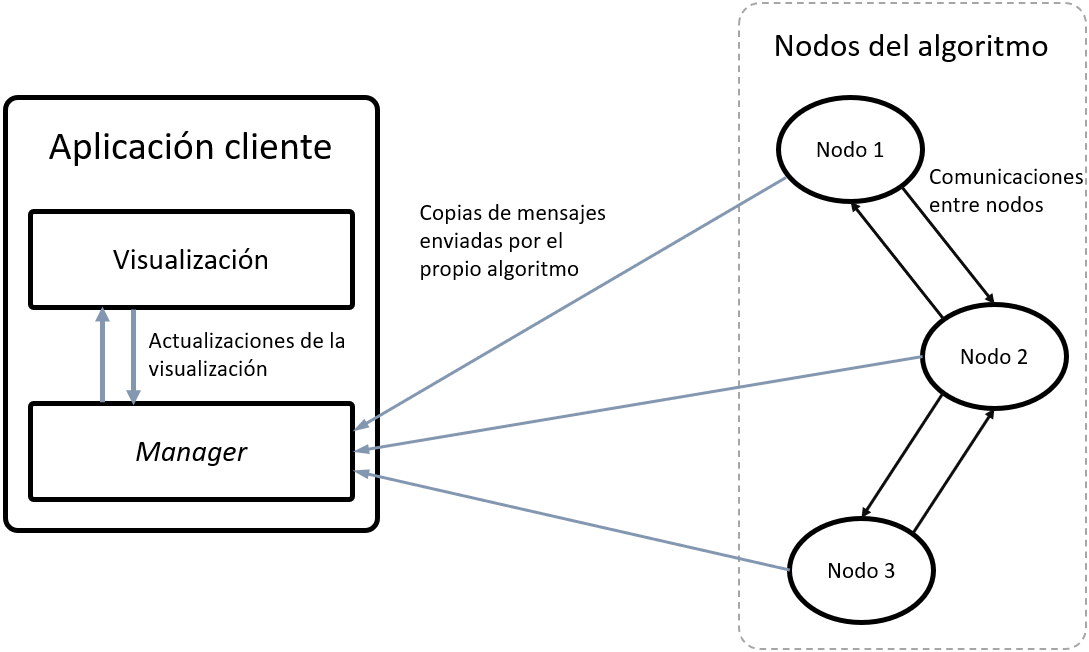
\includegraphics[width=0.7\linewidth]{imagenes/arquitectura1}
  \caption{Diagrama de la primera arquitectura propuesta}
  \label{fig:arquitectura1}
\end{figure}

En la Figura~\ref{fig:arquitectura1} se puede ver en la parte izquierda la aplicación cliente, que se compone de la interfaz, y del proceso \textit{manager} que la actualiza. Ambas partes se ejecutan en la misma máquina. En la parte de la derecha se localizan los nodos del algoritmo, que pueden ejecutarse en un entorno distribuido. Las flechas entre nodos simbolizan las comunicaciones del algoritmo, y las flechas entre cada nodo y el proceso \textit{manager} las copias de los mensajes.

Otra alternativa menos ``intrusiva`` en el algoritmo consiste en modificar de alguna manera las librerías que gestionan los envíos de paquetes de red. De tal forma que el algoritmo llama a la función de librería de envío de mensajes (\texttt{send}, \texttt{sendto}, \texttt{write}, etc) y esta envía una copia del mensaje al proceso \textit{manager}. Esta solución permite no tener que modificar nada del algoritmo. La arquitectura (Figura~\ref{fig:arquitectura2}) es muy parecida a la propuesta anteriormente, lo único que cambia es el origen del envío de las copias de mensajes.

\begin{figure}[h]
  \centering
  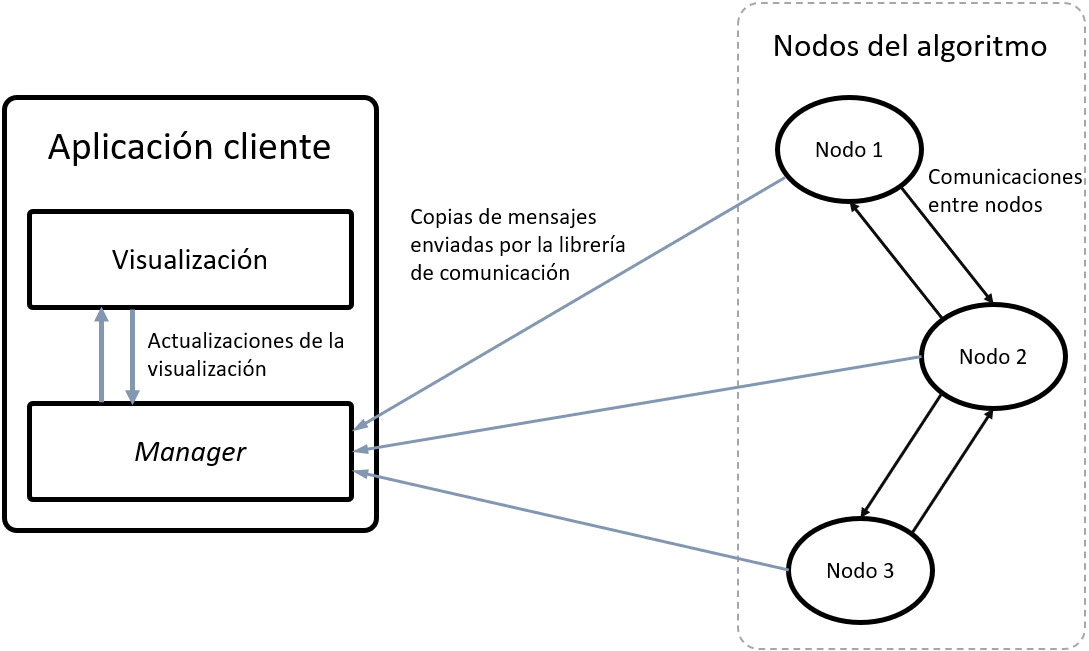
\includegraphics[width=0.7\linewidth]{imagenes/arquitectura2}
  \caption{Diagrama de la segunda arquitectura propuesta}
  \label{fig:arquitectura2}
\end{figure}

\newpage

Sin embargo esta alternativa cuenta con el gran defecto de que no sería posible intercambiar el algoritmo por otro implementado en otro lenguaje de programación cualquiera. Sería necesario volver a modificar las librerías necesarias. Esta resticción, junto con el hecho de que puede ser complicado modificar la funcionalidad incluída en las librerías del lenguaje, motiva la siguiente alternativa.

La alternativa final cuenta con otro proceso capturador o \textit{sniffer} que intercepta el tráfico de red a nivel de protocolo de un determinado proceso. Se ejecuta una instancia junto con cada nodo del algororitmo de tal forma que los mensajes capturados se reenvían al proceso \textit{manager} para que este actualize la visualización. Esta captura de mensajes se lleva a cabo a nivel de protocolo, por lo que no es necesario modificar ningún aspecto del algoritmo que se quiere visualizar. En esta solución el cuadro de mandos se abstrae totalmente del algoritmo, de forma que permite visualizar implementaciones en distrintos lenguajes, siempre que el medio de comunicación sea un protocolo conocido, por ejemplo TCP. Esta modificación se puede observar en la figura~\ref{fig:arquitectura3}.

\begin{figure}[h]
  \centering
  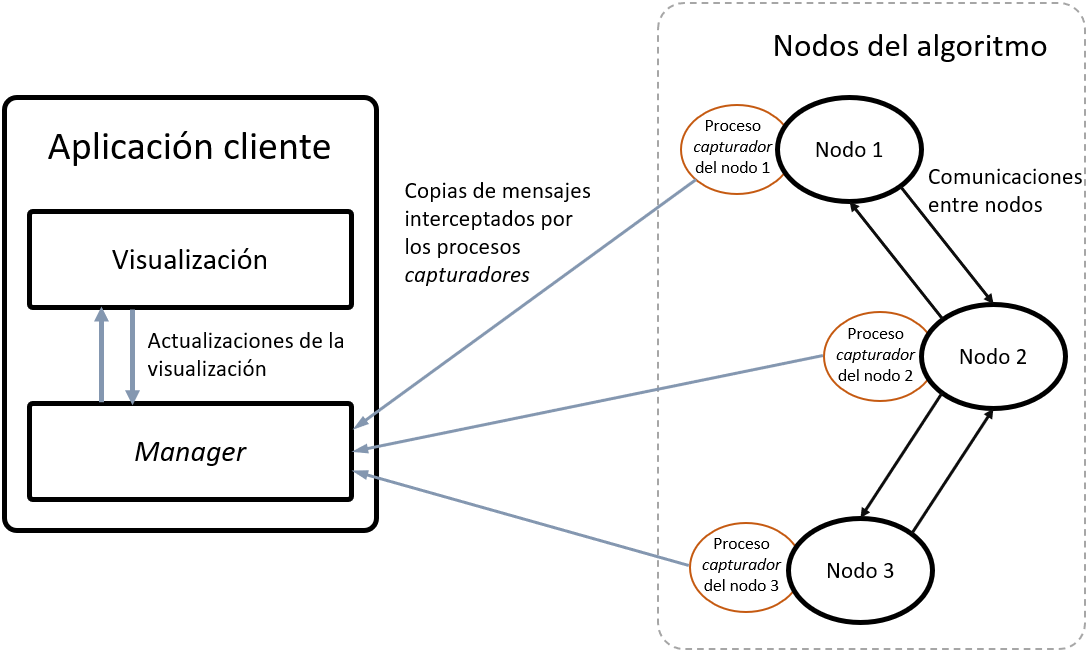
\includegraphics[width=0.7\linewidth]{imagenes/arquitectura3}
  \caption{Diagrama de la tercera arquitectura propuesta}
  \label{fig:arquitectura3}
\end{figure}

Por parte del proceso \textit{manager}, el funcionamiento es el mismo que en las soluciones propuestas anteriormente. Otra ventaja de esta arquitectura es que soportaría también visualizar algoritmos cuyo medio de comunicación se basa en las llamadas a procedimientos remotos (RPC). En las soluciones propuestas anteriores únicamente se tienen en cuenta los algoritmos cuyo modelo de comunicación se basa en el envío de mensajes entre \textit{sockets} (sería necesario modificar el proceso \textit{manger} para admitir la comunicación mediante RPC). Sin embargo, dado que las librerías de llamadas a procedimientos remotos también se basan en la comunicación con algún protocolo (por lo general TCP), también se capturarían estos mensajes.

La ventaja principal de esta arquitectura comparada con las anterior, es que permite un desacoplamiento total del algoritmo. Además de esto, satisface los requisitos que se mencionan en la introducción. A continuación se explicará la implementación detallada de cada uno de los elementos de la arquitectura.

\section{Implementación del algoritmo \texttt{Raft}}

Para la implementación del algoritmo Raft, se ha escogido el lenguaje de programación \textit{Go} \cite{go}, que proporciona numerosas comodidades y ventajas a la hora de programar aplicaciones distribuidas. Por otra parte, la propuesta original de \textit{Raft} \cite{raft1} sugiere que la comunicación entre los nodos se implemente mediante llamadas a procedimientos remotos (RPC) puesto que se elimina la complejidad que supone enviar y recibir mensajes con \textit{sockets}. Sin embargo, en esta implementación, se ha diseñado la comunicación con mensajes tradicionales TCP. Además de que actualmente existen numerosas implementaciones del algoritmo empleando llamadas a procedimientos remotos \cite{raftetcd}\cite{rafteliben}, la ventaja de los mensajes TCP es que es mucho más claro el proceso de envío y recepción de los mensajes.

Además de este aspecto, la implementación incluye la elección de líder completa y la replicación de \textit{log} parcial. La replicación no está completa puesto que esta implementación tiene como objetivo visualizar los mensajes relacionados con el algoritmo, y no el contenido de los \textit{logs} replicados. Por otra parte, la implementación está diseñada para interactuar con cada nodo mediante la entrada estándar del proceso. La función principal de la implementación (\textit{Main}) contiene la lógica necesaria para interactuar con los procesos en segundo plano que ejecutan el algoritmo. Las funcionalidades o comandos que incluye esta implementación son las siguientes:

\begin{itemize}
\item\texttt{START}: Comenzar a ejecutar el algoritmo.
\item\texttt{STOP}: Detiene la ejecución del algoritmo.
\item\texttt{ADD}: Añade un nodo vecino. Se debe suministrar como parámetro la dirección válida del nodo vecino con formato \texttt{ip:puerto}.
\item\texttt{PEERS}: Imprime la lista de nodos vecinos.
\end{itemize}

A continuación se descibe la implementación de cada uno de los componentes del algoritmo. La descripción simplificada de \textit{Raft} puede leerse en el Anexo, o en el artículo original \cite{raft1} (versión completa y detallada). Por otra parte, sólo se muestran partes del código simplificadas que no contienen control de errores.

Cuando un nodo comienza a ejecutar el algoritmo, comienzan a ejecutarse dos procesos secundarios. El primer proceso ejecuta la función \texttt{raft}, que contiene la mayoría del funcionamiento del algoritmo, mientras que el segundo ejecuta la función \texttt{listener}, que es la encargada de recibir mensajes del \textit{socket}. La comunicación entre estas funciones se lleva a cabo mendiante canales de Go \cite{gochannels}, una de las mejores funcionalidades del lenguaje, que son similares a los \textit{pipes} de Linux. El proceso que ejecuta la función \texttt{raft} recibe mensajes de este canal, y en función del estado del nodo y otros factores, actúa de una manera u otra. Por otra parte la función \texttt{listener}, entre otras, envía mensajes al canal.

\subsection{Estado del algoritmo}

El estado del algoritmo se almacena en una estructura con los siguientes campos (se muestran únicamente los relacionados con la descripción del algoritmo):

\begin{lstlisting}[language=go]
type NodeStatus struct {
	peers              []NodeAddr     // Lista de nodos vecinos
	received_votes     int8           // Numero de votos recibidos en una eleccion
	voted_current_term bool           // Indica si se ha votado en el term acutal
	term               int            // Term actual
	log                []NodeLogEntry // Lista de entradas de log
	raftStatus         uint8          // Estado de raft: follower | candidate | leader
	electionTimeout    int64          // Tiempo de timeout para listener()
	leaderHeartbeat    int64          // Intervalo de tiempo entre mensajes para leaderHeartbeats()
	eventChan          chan Event     // Canal de comunicacion
}
\end{lstlisting}

\subsection{Implementación de \texttt{listener}}

La implementación de la función \texttt{listener} es simple:

\begin{lstlisting}[language=go]
func listener(l *net.TCPListener, status *NodeStatus) {
	for {
		var timeout time.Time
		
		// Calcular en que instante habra timeout
		timeout = time.Now().Add(time.Millisecond * time.Duration(status.electionTimeout))
		
		// Establecer el timeout para el socket
		l.SetDeadline(timeout)

		// Esperar a una nueva conexion
		conn, err := l.Accept()
		if err != nil {
			if errors.Is(err, os.ErrDeadlineExceeded) {
				if status.raftStatus == candidate || status.raftStatus == follower {
					// Si se ha superado el timeout y el estado es candidate o follower
					// Escribir en el canal el evento de timeout
					status.eventChan <- Event{
						msg: NodeMsg{MsgType: followerTimeout},
					}
				} else {
					// Si es lider entonces este timeout no le afecta
				}
				continue
		}
		
		// Procesar la nueva conexion
		go responseHandler(conn, status)
	}
}
\end{lstlisting}

A esta función se le pasa como parámetro el estado del nodo, y el socket por el que el nodo recibe mensajes. A modo de resumen, la funcionalidad se basa en esperar a recibir una nueva conexión en el \textit{socket} y procesar el mensaje con la función \texttt{responseHandler}, o bien enviar el evento de \textit{timeout} al canal de comunicación en el caso de que no se inicie una conexión en un tiempo determinado.

\subsection{Implementación de \texttt{responseHandler}}

La implementación de la función \texttt{responseHandler} es la siguiente:

\begin{lstlisting}[language=go]
func responseHandler(conn net.Conn, status *NodeStatus) {
	decoder := json.NewDecoder(conn)
	defer conn.Close()

	var msg NodeMsg
	decoder.Decode(&msg)
	
	status.eventChan <- Event{
		msg:    msg,
		sender: conn.RemoteAddr().(*net.TCPAddr).IP.String(),
	}
}
\end{lstlisting}

Esta función recibe del \textit{socket} un mensaje, lo deserializa a un \texttt{struct} de Go \cite{gostructs} y envía este objeto al canal.

\subsection{Implementación de \texttt{raft}}

La función que lee y procesa los mensajes del canal es \texttt{raft}, que implementa la mayoría de las funcionalidades del algoritmo.

\begin{lstlisting}[language=go]
func raft(wg *sync.WaitGroup, status *NodeStatus) {
	// Leer eventos del canal
	for event := range status.eventChan {
		switch event.msg.MsgType {
		// Si otro nodo ha comenzado una votacion		
		case requestVote:
			// Independientemente del estado, convertirse en follower si el term del mensaje es superior y si no se ha votado en el term actual
			if event.msg.Term > status.term && !status.voted_current_term {
				status.voted_current_term = true
				status.raftStatus = follower
				status.term = event.msg.Term
				go sendMsg(
					NodeMsg{MsgType: grantVote, Term: event.msg.Term},
					event.sender,
					event.msg.SenderPort,
				)
			}
		// Si es un mensaje de voto aceptado
		case grantVote:
			switch status.raftStatus {
			case follower:
				// No hace nada porque ya se termino la eleccion
			case candidate:
				// Mirar si es un voto a nuestra eleccion
				if event.msg.Term == status.term {
					status.received_votes++
					if int(status.received_votes) > (len(status.peers)+1)/2 {
						// Si se han recibido suficientes votos, convertirse en lider
						status.raftStatus = leader
						go leaderHeartbeats(status)
					}
				}
			case leader:
				// No hacer nada porque ya se ha conseguido ser lider
			}
		// Si es un mensaje con entradas de log
		case appendEntries:
			if event.msg.Term > status.term {
				// Si el term del mensaje es superior, convertirse en follower
				status.voted_current_term = false
				status.raftStatus = follower
				status.term = event.msg.Term
			}
		// Si es un evento de timeout
		case followerTimeout:
			switch status.raftStatus {
			case follower, candidate:
				// Comenzar eleccion si es follower o candidate
				go startElection(status)
			case leader:
				// Ignorar evento
			}
		}
	}
}
\end{lstlisting}

Como se puede observar, esta función altera el estado del algoritmo en función de los mensajes que recibe del canal y del estado en el que se encuentra:

\begin{itemize}
\item Cuando el mensaje que recibe es de tipo \texttt{requestVote}, significa que algún otro nodo ha iniciado una votación. En este escenario, el nodo se convertirá en seguidor si el nuevo \textit{term} es superior, y si no ha votado todavía en el \textit{term} actual.

\item En el caso de que el mensaje recibido sea de tipo \texttt{grantVote}, significa que el propio nodo ha inciado una votación anteriormente, y algún otro nodo ha aceptado el voto. Si el nodo está en el estado \textit{follower}, se ignora la petición, puesto que la votación se ha terminado y no se ha conseguido el liderazgo. En el caso en el que el estado del nodo sea \textit{candidate}, hay que comprobar si el voto aceptado es de la votación actual. En el caso de que lo sea, el nodo se convierte en líder ejecutando la función \texttt{leaderHeartbeats}. En el caso de que el estado sea \textit{leader}, se ignora el mensaje, puesto que ya se ha conseguido el liderazgo.

\item En el caso de que se reciba un mensaje de tipo \texttt{appendEntries}, el nodo se convierte en seguidor si el \texttt{term} del mensaje es superior al term actual.

\item Si el tipo del mensaje es \texttt{followerTimeout}, significa que la función \texttt{listener} no ha recibido una nueva conexión en el tiempo del \textit{timeout}. Este escenario implica que el nodo inicie una votación (función \texttt{startElection}) en el caso de que sea seguidor o candidato.
\end{itemize}

\subsection{Implementación de \texttt{leaderHeartbeats}}

La función \texttt{leaderHeartbeats} se ejecuta cuando el estado del nodo es \texttt{leader}. El objetivo es enviar periódicamente mensajes de tipo \texttt{appendEntries} a los nodos vecinos para que continúen en el estado \textit{follower}. Sólamente termina cuando el estado del nodo deja de ser \textit{leader}. 

\begin{lstlisting}[language=go]
func leaderHeartbeats(status *NodeStatus) {
	for {
		if status.raftStatus != leader {
			return
		}

		msg := NodeMsg{
			MsgType:    appendEntries,
			Term:       status.term,
			Entries:    nil,
		}
		timeout := status.leaderHeartbeat
		
		// Enviar appendEntries a los vecinos
		for _, p := range status.peers {
			go sendMsg(msg, p.ip, p.port)
		}

		// Esperar para enviar la siguiente rafaga de appendEntries
		<-time.After(time.Duration(timeout) * time.Millisecond)
	}
}
\end{lstlisting}

\subsection{Implementación de \texttt{startElection}}

Por último, la función \texttt{startElection} es la encargada de enviar mensajes de tipo \texttt{requestVote} a los nodos vecinos cuando se inicia una nueva elección. 

\begin{lstlisting}[language=go]
func startElection(status *NodeStatus) {
	status.raftStatus = candidate
	status.term++
	status.received_votes = 1 // Votar por uno mismo

	msg := NodeMsg{
		MsgType:    requestVote,
		Term:       status.term,
		Entries:    nil,
	}

	for _, p := range status.peers {
		go sendMsg(msg, p.ip, p.port)
	}
}
\end{lstlisting}

\section{Implementación del proceso \textit{capturador}}

Como se describe en la sección~\ref{sec:arquitectura}, el proceso capturador debe capturar los mensajes de red que envía el nodo y reenviarlos al proceso manager. Además de esto, para permitir una comunicación bidireccional, debe ser capaz de interactuar con el proceso que ejecuta el algoritmo.

\begin{itemize}
\item Explicar que no se pueden hacer sockets raw de python en windows
\item Poner el codigo de sniffer.py
\item Explicar los mensajes de ADD
\end{itemize}

\section{Implementación y descripción del cliente}

El cliente es la aplicación que ejecuta la interfaz de usuario.

\begin{itemize}
\item Explicar eleccion de elecctron/js
\item Explicar libreria vis.js
\item Explicar restricciones de vis.js
\item Explicar funcionamiento\\
\item Explicar la relacion entre los botones y los mensajes enviados al sniffer.
\end{itemize}

\section{Implementación del \textit{manager}}

\begin{itemize}
\item Explicar que esta dentro de la interfaz
\item Poner el codigo y explicar
\end{itemize}

\section{Caso de uso}

En este apartado se demuestra la funcionalidad completa de la aplicación con un algoritmo concreto: Raft. El funcionamiento de este algoritmo se puede encontrar en el Anexo de este documento. A modo de resumen, Raft es un algoritmo de consenso empleado para replicar información en conjunto de nodos.


